\documentclass[11pt]{report}

\usepackage{amsmath}
\usepackage{graphicx}
\usepackage{braket}
\usepackage{mathtools}
\usepackage{slashed}
\usepackage{amsfonts}
\usepackage{cancel}
\usepackage{a4wide}
\usepackage{caption}
\usepackage{subcaption}

\title{Modeling and Simulation Hand-In 2}
\author{Georgios Smyridis}
\date{}

\begin{document}

\maketitle

\section*{Exercise 5}

\subsection*{Question a)}
The code for the change\_volume() is attached with the report. The change\_volume() attempts to change the volume by a random number within a range. Then, it scales the box and the positions accordingly. After that, it checks for overlaps. If there are overlaps, it rejects the volume change and simply returns zero. If, on the other hand, there are no overlaps, it accepts the volume change ba	sed on the acceptance rule derived in the class, but modified for the dynamics of our system.
\begin{align}
	acc(o\rightarrow n) = \text{min}\bigg(1,\ \exp\bigg[-\beta(V_{new}-V_{old})+N\log\frac{V_{new}}{V_{old}}\bigg]\bigg)
\end{align}

\subsection*{Question b)}

After we have created the change\_volume() function, we perform a Monte Carlo Simulation for the NPT ensemble. After a set number of steps, we "measure" the average volume of the system and we plot it across the entire simulation run. We notice that in the beginning the volume flactuates a lot, while after a number of steps is stabilises and doesn't fluctuate a lot. This is because the system has reached equilibrium. The rate of acceptance in this state depends on the choice of maximum volume change that we have chosen. We choose to run the simulation with a maximum volume change that leads to acceptance rate 0.4 to 0.6 at equilibrium. We repeat the simulation with starting configuration an FCC crystal and decreasing the pressure starting from 50 (see Figure 1 red line). Then we start from a liquid configuration and increase the pressure gradually (see Figure 1 blue line).

\subsection*{Question c)}

Finally, we compare with the Carnahan-Starling equation (see Figure 1 green line) with the results retrieved from the simulations, in Figure 1.

\begin{figure*}[ht!]
	\begin{center}
		\includegraphics[scale = 0.4]{packing}
		\caption{Packing fraction vs reduced pressure. The horizontal axis is reduced pressure, and the vertical the packing fraction. The red line represents the results for the crystalic phase, the blue for the liquid phase, and the green the Carnahan-Starling equation.}
	\end{center}
\end{figure*}




\section*{Exercise 6}

\subsection*{Question a)}

The radial distribution function (RDF) is a measure of the probability of finding a particle in distance $r$ from any other particle compared to the same probability for an ideal gas. As the distance between particles becomes very large and the density very low, the system becomes increasingly homogeneous at large distances, and the probability of finding another particle at any given distance becomes equal to the probability of finding one in an ideal gas. Therefore, the radial distribution function becomes unity.

\subsection*{Question b)}

It is easy to write a function that calculates the distances among all pairs of particles, assign them to a bin and then divide by the number $n_{id}(b)$. I then use this function in the following way. If one assumes that the volume of each particle is one, then packing fraction and the density of the particles can be made to be the same. Therefore, setting different packing fractions is equivalent to setting different densities. Then, we run an NVT Monte Carlo simulation, making sure that the acceptance rate of moves is 0.4 to 0.6. At the end,  we calculate the radial distribution function histogram. Since running it only once for each density value produces a histogram that is prone to "noice", i.e. it's only one sample. Therefore, for each density value, one should calculate the histogram multiple times and then average. The results for densities (packing fractions) 0.2, 0.4 and 0.6 are depicted in Figure %TODO add figure'

\subsection*{Question c)}

From the plots, one can immediately notice three things. First, as the density (packing fraction) increases, the RDF assumes a higher value for shorter distances. This makes sense, since since the box is more packed and the average distance between the particles decreases. This translates into higher probability of finding particles in close proximity. The second thing that is immediately apparent, is that for higher densities, the distribution decays faster. Again, this behaviour is logical. In higher densities, it is less likely to find particles at large distances. Finally, one can observe that the distribution becomes less and less smooth. This happens because, in lower densities, the average distance between particles increases and it results in a more evenly distributed probability of finding particles in different distances from each other.

\begin{figure}[ht!]
     \centering
     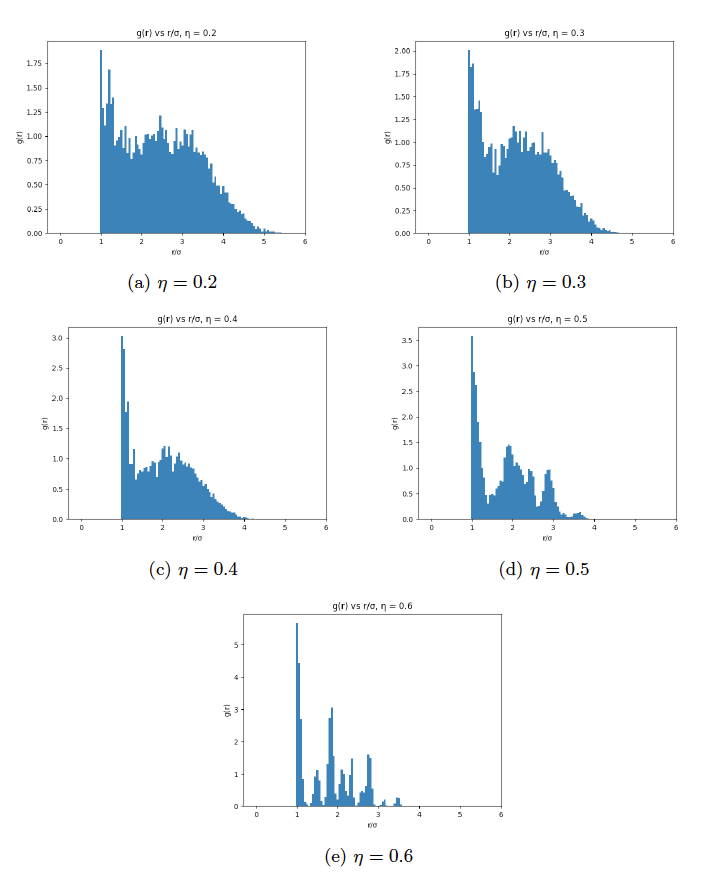
\includegraphics{pc_NVT.png}

\end{figure}




\end{document}
